\documentclass{standalone}
\usepackage[T1]{fontenc}
\usepackage[utf8]{inputenc}
\usepackage{pgf,tikz}
\usepackage{setspace}
\usepackage{pgfplots}
\usepgfplotslibrary{groupplots}

\pgfplotsset{compat=1.12}

% Style to select only points from #1 to #2 (inclusive)
\pgfplotsset{select coords between index/.style 2 args={
    x filter/.code={
        \ifnum\coordindex<#1\def\pgfmathresult{}\fi
        \ifnum\coordindex>#2\def\pgfmathresult{}\fi
    }
}}


\def\axlim{5}
\begin{document}

  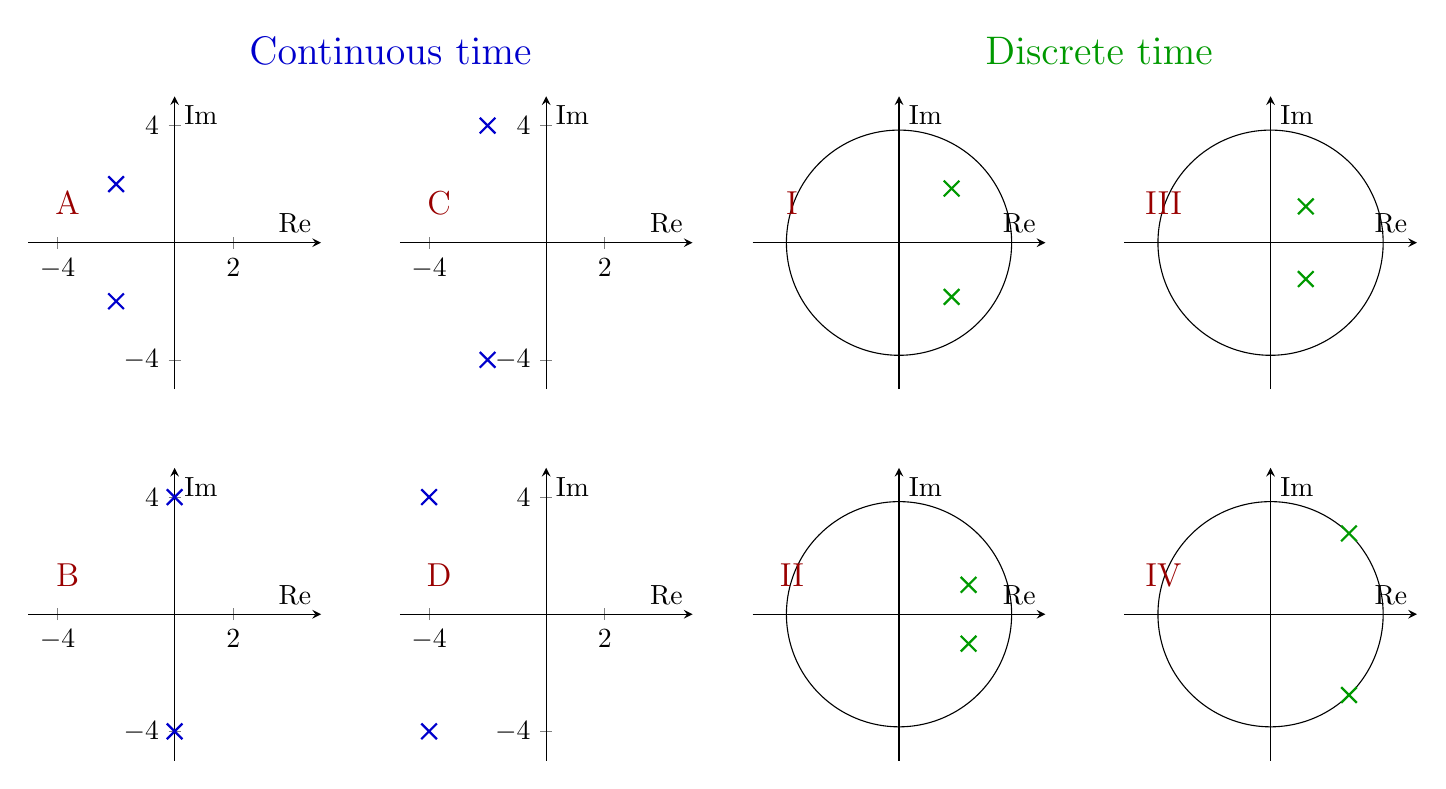
\begin{tikzpicture}[node distance=2cm]
    \pgfmathsetmacro{\hh}{0.2}
    \pgfmathsetmacro{\realone}{-2}
    \pgfmathsetmacro{\imone}{2}
    \pgfmathsetmacro{\realtwo}{-2}
    \pgfmathsetmacro{\imtwo}{4}
    \pgfmathsetmacro{\realthree}{0}
    \pgfmathsetmacro{\imthree}{4}
    \pgfmathsetmacro{\realfour}{-4}
    \pgfmathsetmacro{\imfour}{4}

    \pgfmathsetmacro{\magone}{exp(\realone*\hh)}
    \pgfmathsetmacro{\argone}{\imone*\hh*180/3.14}
    \pgfmathsetmacro{\realoned}{\magone*cos(\argone)}
    \pgfmathsetmacro{\imoned}{\magone*sin(\argone)}

    \pgfmathsetmacro{\magtwo}{exp(\realtwo*\hh)}
    \pgfmathsetmacro{\argtwo}{\imtwo*\hh*180/3.14}
    \pgfmathsetmacro{\realtwod}{\magtwo*cos(\argtwo)}
    \pgfmathsetmacro{\imtwod}{\magtwo*sin(\argtwo)}

    \pgfmathsetmacro{\magthree}{exp(\realthree*\hh)}
    \pgfmathsetmacro{\argthree}{\imthree*\hh*180/3.14}
    \pgfmathsetmacro{\realthreed}{\magthree*cos(\argthree)}
    \pgfmathsetmacro{\imthreed}{\magthree*sin(\argthree)}

    \pgfmathsetmacro{\magfour}{exp(\realfour*\hh)}
    \pgfmathsetmacro{\argfour}{\imfour*\hh*180/3.14}
    \pgfmathsetmacro{\realfourd}{\magfour*cos(\argfour)}
    \pgfmathsetmacro{\imfourd}{\magfour*sin(\argfour)}

    \begin{scope}[xshift=0, yshift=0]
      \node {\Large \textcolor{blue!80!black}{Continuous time}};
    \end{scope}
    
    \begin{scope}[xshift=-4.6cm, yshift=-4.3cm]

      \begin{groupplot} [
        group style={
          group name=poles,
          group size=2 by 2,
          xlabels at=all}, 
        height=5.3cm, width=5.3cm,
        axis lines=middle,
        % grid=both,
        % ytick=\empty,
        ytick={-4, 4}, 
        xtick={-4, 2},
        % xtick=\empty,
        % xticklabel=$a$,
        xlabel=Re,
        ylabel=Im,
        xmin=-\axlim, xmax=\axlim,
        ymin=-\axlim, ymax=\axlim,
        % only marks,
        ]
        
        \nextgroupplot   
        \addplot[thick, blue!80!black, mark=x, mark size=4pt, only marks,] coordinates { (\realone, \imone) (\realone, -\imone) };
        % \addplot[mark=o, mark size=4pt, only marks, select coords between index={0}{0}]  table {apollo-lead-zeros-case1.txt};

        \nextgroupplot   
        \addplot[thick, blue!80!black, mark=x, mark size=4pt, only marks,] coordinates { (\realtwo, \imtwo) (\realtwo, -\imtwo) };
        % \addplot[mark=o, mark size=4pt, only marks]  table {apollo-lead-zeros-case2.txt};

        \nextgroupplot   
        \addplot[thick, blue!80!black, mark=x, mark size=4pt, only marks,] coordinates { (\realthree, \imthree) (\realthree, -\imthree) };
        % \addplot[mark=o, mark size=4pt, only marks]  table {apollo-lead-zeros-case3.txt};

        \nextgroupplot   
        \addplot[thick, blue!80!black, mark=x, mark size=4pt, only marks,] coordinates { (\realfour, \imfour) (\realfour, -\imfour) };

        % \addplot[mark=o, mark size=4pt, only marks]  table {apollo-lead-zeros-case4.txt};

      \end{groupplot}


      \node at ($ (poles c1r1.west) + (5mm, 5mm) $) {\large \textcolor{red!60!black!}{A}};
      \node at ($ (poles c1r2.west) + (5mm, 5mm) $) {\large \textcolor{red!60!black!}{B}};
      \node at ($ (poles c2r1.west) + (5mm, 5mm) $) {\large \textcolor{red!60!black!}{C}};
      \node at ($ (poles c2r2.west) + (5mm, 5mm) $) {\large \textcolor{red!60!black!}{D}};
    \end{scope}


    \begin{scope}[xshift=9cm, yshift=0]
      \node {\Large \textcolor{green!60!black}{Discrete time}};
    \end{scope}
    
    \begin{scope}[xshift=4.6cm, yshift=-4.3cm]

      \begin{groupplot} [
        group style={
          group name=poles,
          group size=2 by 2,
          xlabels at=all}, 
        height=5.3cm, width=5.3cm,
        axis lines=middle,
        % grid=both,
        % ytick=\empty,
        ytick={-4, 4}, 
        xtick={-4, 2},
        % xtick=\empty,
        % xticklabel=$a$,
        xlabel=Re,
        ylabel=Im,
        xmin=-1.3, xmax=1.3,
        ymin=-1.3, ymax=1.3,
        % only marks,
        ]
        
        \nextgroupplot   
        \addplot[thick, green!60!black, mark=x, mark size=4pt, only marks,] coordinates { (\realtwod, \imtwod) (\realtwod, -\imtwod) };
        \addplot[ thin, smooth, domain=0:360, samples=200,] plot ({cos(x)}, {sin(x)}); 
        % \addplot[mark=o, mark size=4pt, only marks, select coords between index={0}{0}]  table {apollo-lead-zeros-case1.txt};

        \nextgroupplot   
        \addplot[thick, green!60!black, mark=x, mark size=4pt, only marks,] coordinates { (\realfourd, \imfourd) (\realfourd, -\imfourd) };
        \addplot[ thin, smooth, domain=0:360, samples=200,] plot ({cos(x)}, {sin(x)}); 
        % \addplot[mark=o, mark size=4pt, only marks]  table {apollo-lead-zeros-case2.txt};

        \nextgroupplot   
        \addplot[thick, green!60!black, mark=x, mark size=4pt, only marks,] coordinates { (\realoned, \imoned) (\realoned, -\imoned) };
        \addplot[ thin, smooth, domain=0:360, samples=200,] plot ({cos(x)}, {sin(x)}); 
        %\draw (axis cs:0,0) circle [radius=1];
        
        \nextgroupplot   
        \addplot[thick, green!60!black, mark=x, mark size=4pt, only marks,] coordinates { (\realthreed, \imthreed) (\realthreed, -\imthreed) };
        \addplot[ thin, smooth, domain=0:360, samples=200,] plot ({cos(x)}, {sin(x)}); 

        % \addplot[mark=o, mark size=4pt, only marks]  table {apollo-lead-zeros-case4.txt};

      \end{groupplot}


      \node at ($ (poles c1r1.west) + (5mm, 5mm) $) {\large \textcolor{red!60!black!}{I}};
      \node at ($ (poles c1r2.west) + (5mm, 5mm) $) {\large \textcolor{red!60!black!}{II}};
      \node at ($ (poles c2r1.west) + (5mm, 5mm) $) {\large \textcolor{red!60!black!}{III}};
      \node at ($ (poles c2r2.west) + (5mm, 5mm) $) {\large \textcolor{red!60!black!}{IV}};
    \end{scope}


\end{tikzpicture}
\end{document}
